\documentclass{standalone}
\usepackage{amsmath}
\usepackage{bm}
\usepackage[dvipsnames]{xcolor}

\usepackage{tikz}
\usetikzlibrary{positioning,arrows.meta,backgrounds,shapes}
\usetikzlibrary{matrix}

\definecolor{body}{HTML}{5b84b1}
\definecolor{tail}{HTML}{fc766a}

\begin{document}

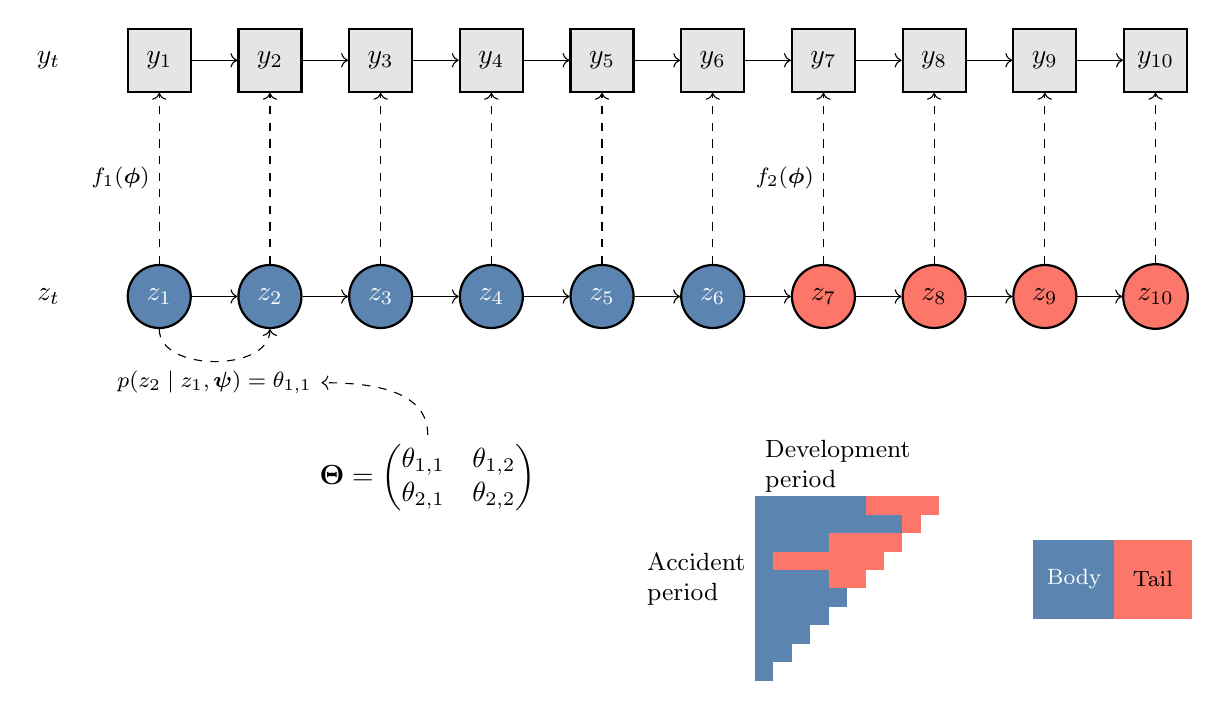
\begin{tikzpicture}[
    base/.style = {circle, thick, node distance = 4em, draw=black, minimum size=0.8cm},
    state1/.style = {base, fill=body, text=white},
    state2/.style = {base, fill=tail},
    observed1/.style = {rectangle, ultra thin, fill=body},
    observed2/.style = {rectangle, ultra thin, fill=tail},
    observed/.style = {base, rectangle, fill=black!10!white},
]

    % latents
    \node[fill=white] (zbase) {$z_{t}$};
    \node[state1, right of = zbase] (z1) {$z_{1}$};
    \node[state1, right of = z1] (z2) {$z_{2}$};
    \node[state1, right of = z2] (z3) {$z_{3}$};
    \node[state1, right of = z3] (z4) {$z_{4}$};
    \node[state1, right of = z4] (z5) {$z_{5}$};
    \node[state1, right of = z5] (z6) {$z_{6}$};
    \node[state2, right of = z6] (z7) {$z_{7}$};
    \node[state2, right of = z7] (z8) {$z_{8}$};
    \node[state2, right of = z8] (z9) {$z_{9}$};
    \node[state2, right of = z9] (z10) {$z_{10}$};

    % observed
    \node[fill=white, above of = zbase, yshift=2cm] (ybase) {$y_{t}$};
    \node[observed, right of = ybase] (y1) {$y_{1}$};
    \node[observed, right of = y1] (y2) {$y_2$};
    \node[observed, right of = y2] (y3) {$y_3$};
    \node[observed, right of = y3] (y4) {$y_4$};
    \node[observed, right of = y4] (y5) {$y_5$};
    \node[observed, right of = y5] (y6) {$y_6$};
    \node[observed, right of = y6] (y7) {$y_7$};
    \node[observed, right of = y7] (y8) {$y_8$};
    \node[observed, right of = y8] (y9) {$y_9$};
    \node[observed, right of = y9] (y10) {$y_{10}$};

    % flows
    \draw[->] (z1) -- (z2);
    \draw[->, dashed] (z1) to [out=270, in=270] node[below, font=\footnotesize] (theta) {$p(z_{2} \mid z_{1}, \bm{\psi}) = \theta_{1,1}$} (z2);
    \draw[->] (z2) -- (z3);
    \draw[->] (z3) -- (z4);
    \draw[->] (z4) -- (z5);
    \draw[->] (z5) -- (z6);
    \draw[->] (z6) -- (z7);
    \draw[->] (z7) -- (z8);
    \draw[->] (z8) -- (z9);
    \draw[->] (z9) -- (z10);
    \draw[->] (y1) -- (y2);
    \draw[->] (y2) -- (y3);
    \draw[->] (y3) -- (y4);
    \draw[->] (y4) -- (y5);
    \draw[->] (y5) -- (y6);
    \draw[->] (y6) -- (y7);
    \draw[->] (y7) -- (y8);
    \draw[->] (y8) -- (y9);
    \draw[->] (y9) -- (y10);


	% matrices
	\node[below right of = theta, yshift=-0.5cm, xshift=2cm] (tm) {$\begin{aligned}
			\mathbf{\Theta} = \begin{pmatrix} 
				\theta_{1,1} & \theta_{1,2}\\ 
				\theta_{2,1} & \theta_{2, 2} 
			\end{pmatrix}
		\end{aligned}
	$};
	\draw[dashed, ->] (tm) to[in=360, out=90] (theta);

    % triangle
    \matrix (triangle) [
        matrix of nodes, 
        nodes in empty cells, 
        in front of path, 
        ampersand replacement = \&, 
        below right of = z6, 
        xshift=1cm,
        yshift=-3cm
    ]
    {
        % row 1
        \node[observed1] {}; \&
        \node[observed1] {}; \&
        \node[observed1] {}; \&
        \node[observed1] {}; \&
        \node[observed1] (col5) {}; \&
        \node[observed1] {}; \&
        \node[observed2] {}; \&
        \node[observed2] {}; \&
        \node[observed2] {}; \&
        \node[observed2] {}; \\
        % row 2
        \node[observed1] {}; \&
        \node[observed1] {}; \&
        \node[observed1] {}; \&
        \node[observed1] {}; \&
        \node[observed1] {}; \&
        \node[observed1] {}; \&
        \node[observed1] {}; \&
        \node[observed1] {}; \&
        \node[observed2] {}; \\
        % row 3
        \node[observed1] {}; \&
        \node[observed1] {}; \&
        \node[observed1] {}; \&
        \node[observed1] {}; \&
        \node[observed2] {}; \&
        \node[observed2] {}; \&
        \node[observed2] {}; \&
        \node[observed2] {}; \\
        % row 4
        \node[observed1] {}; \&
        \node[observed2] {}; \&
        \node[observed2] {}; \&
        \node[observed2] {}; \&
        \node[observed2] {}; \&
        \node[observed2] {}; \&
        \node[observed2] {}; \\
        % row 5
        \node[observed1] {}; \&
        \node[observed1] {}; \&
        \node[observed1] {}; \&
        \node[observed1] {}; \&
        \node[observed2] (row5) {}; \&
        \node[observed2] {}; \\
        % row 6
        \node[observed1] {}; \&
        \node[observed1] {}; \&
        \node[observed1] {}; \&
        \node[observed1] {}; \&
        \node[observed1] {}; \\
        % row 7
        \node[observed1] {}; \&
        \node[observed1] {}; \&
        \node[observed1] {}; \&
        \node[observed1] {}; \\
        % row 8
        \node[observed1] {}; \&
        \node[observed1] {}; \&
        \node[observed1] {}; \\
        % row 9
        \node[observed1] {}; \&
        \node[observed1] {}; \\
        % row 10
        \node[observed1] {}; \\
    };

    % triangle labels
    \node [left of = row5, font=\small, align=left, xshift=-0.8cm] (xlabel) {Accident\\ period};
    \node [above of = col5, font=\small, align=left, yshift=-0.5cm] (ylabel) {Development\\ period};
    \node [observed1, right of = row5, xshift=2cm, text=white, minimum size=1cm, font=\footnotesize, inner sep=5pt] (body) {Body};
    \node [observed2, right of = body, font=\footnotesize, minimum size=1cm, inner sep=5pt] (tail) {Tail};

    % mappings
    \draw[->, dashed] (z1) -- node[left, font=\footnotesize] (fx) {$f_{1}(\bm{\phi})$} (y1);
    \draw[->, dashed] (z2) -- (y2);
    \draw[->, dashed] (z3) -- (y3);
    \draw[->, dashed] (z4) -- (y4);
    \draw[->, dashed] (z5) -- (y5);
    \draw[->, dashed] (z6) -- (y6);
    \draw[->, dashed] (z7) -- node[left, font=\footnotesize] (f2x) {$f_{2}(\bm{\phi})$} (y7);
    \draw[->, dashed] (z8) -- (y8);
    \draw[->, dashed] (z9) -- (y9);
    \draw[->, dashed] (z10) -- (y10);

\end{tikzpicture}
\end{document}
